% Options for packages loaded elsewhere
% Options for packages loaded elsewhere
\PassOptionsToPackage{unicode}{hyperref}
\PassOptionsToPackage{hyphens}{url}
\PassOptionsToPackage{dvipsnames,svgnames,x11names}{xcolor}
%
\documentclass[
  letterpaper,
  DIV=11,
  numbers=noendperiod]{scrreprt}
\usepackage{xcolor}
\usepackage{amsmath,amssymb}
\setcounter{secnumdepth}{5}
\usepackage{iftex}
\ifPDFTeX
  \usepackage[T1]{fontenc}
  \usepackage[utf8]{inputenc}
  \usepackage{textcomp} % provide euro and other symbols
\else % if luatex or xetex
  \usepackage{unicode-math} % this also loads fontspec
  \defaultfontfeatures{Scale=MatchLowercase}
  \defaultfontfeatures[\rmfamily]{Ligatures=TeX,Scale=1}
\fi
\usepackage{lmodern}
\ifPDFTeX\else
  % xetex/luatex font selection
\fi
% Use upquote if available, for straight quotes in verbatim environments
\IfFileExists{upquote.sty}{\usepackage{upquote}}{}
\IfFileExists{microtype.sty}{% use microtype if available
  \usepackage[]{microtype}
  \UseMicrotypeSet[protrusion]{basicmath} % disable protrusion for tt fonts
}{}
\makeatletter
\@ifundefined{KOMAClassName}{% if non-KOMA class
  \IfFileExists{parskip.sty}{%
    \usepackage{parskip}
  }{% else
    \setlength{\parindent}{0pt}
    \setlength{\parskip}{6pt plus 2pt minus 1pt}}
}{% if KOMA class
  \KOMAoptions{parskip=half}}
\makeatother
% Make \paragraph and \subparagraph free-standing
\makeatletter
\ifx\paragraph\undefined\else
  \let\oldparagraph\paragraph
  \renewcommand{\paragraph}{
    \@ifstar
      \xxxParagraphStar
      \xxxParagraphNoStar
  }
  \newcommand{\xxxParagraphStar}[1]{\oldparagraph*{#1}\mbox{}}
  \newcommand{\xxxParagraphNoStar}[1]{\oldparagraph{#1}\mbox{}}
\fi
\ifx\subparagraph\undefined\else
  \let\oldsubparagraph\subparagraph
  \renewcommand{\subparagraph}{
    \@ifstar
      \xxxSubParagraphStar
      \xxxSubParagraphNoStar
  }
  \newcommand{\xxxSubParagraphStar}[1]{\oldsubparagraph*{#1}\mbox{}}
  \newcommand{\xxxSubParagraphNoStar}[1]{\oldsubparagraph{#1}\mbox{}}
\fi
\makeatother


\usepackage{longtable,booktabs,array}
\newcounter{none} % for unnumbered tables
\usepackage{calc} % for calculating minipage widths
% Correct order of tables after \paragraph or \subparagraph
\usepackage{etoolbox}
\makeatletter
\patchcmd\longtable{\par}{\if@noskipsec\mbox{}\fi\par}{}{}
\makeatother
% Allow footnotes in longtable head/foot
\IfFileExists{footnotehyper.sty}{\usepackage{footnotehyper}}{\usepackage{footnote}}
\makesavenoteenv{longtable}
\usepackage{graphicx}
\makeatletter
\newsavebox\pandoc@box
\newcommand*\pandocbounded[1]{% scales image to fit in text height/width
  \sbox\pandoc@box{#1}%
  \Gscale@div\@tempa{\textheight}{\dimexpr\ht\pandoc@box+\dp\pandoc@box\relax}%
  \Gscale@div\@tempb{\linewidth}{\wd\pandoc@box}%
  \ifdim\@tempb\p@<\@tempa\p@\let\@tempa\@tempb\fi% select the smaller of both
  \ifdim\@tempa\p@<\p@\scalebox{\@tempa}{\usebox\pandoc@box}%
  \else\usebox{\pandoc@box}%
  \fi%
}
% Set default figure placement to htbp
\def\fps@figure{htbp}
\makeatother





\setlength{\emergencystretch}{3em} % prevent overfull lines

\providecommand{\tightlist}{%
  \setlength{\itemsep}{0pt}\setlength{\parskip}{0pt}}



 


\KOMAoption{captions}{tableheading}
\makeatletter
\@ifpackageloaded{bookmark}{}{\usepackage{bookmark}}
\makeatother
\makeatletter
\@ifpackageloaded{caption}{}{\usepackage{caption}}
\AtBeginDocument{%
\ifdefined\contentsname
  \renewcommand*\contentsname{Table of contents}
\else
  \newcommand\contentsname{Table of contents}
\fi
\ifdefined\listfigurename
  \renewcommand*\listfigurename{List of Figures}
\else
  \newcommand\listfigurename{List of Figures}
\fi
\ifdefined\listtablename
  \renewcommand*\listtablename{List of Tables}
\else
  \newcommand\listtablename{List of Tables}
\fi
\ifdefined\figurename
  \renewcommand*\figurename{Figure}
\else
  \newcommand\figurename{Figure}
\fi
\ifdefined\tablename
  \renewcommand*\tablename{Table}
\else
  \newcommand\tablename{Table}
\fi
}
\@ifpackageloaded{float}{}{\usepackage{float}}
\floatstyle{ruled}
\@ifundefined{c@chapter}{\newfloat{codelisting}{h}{lop}}{\newfloat{codelisting}{h}{lop}[chapter]}
\floatname{codelisting}{Listing}
\newcommand*\listoflistings{\listof{codelisting}{List of Listings}}
\makeatother
\makeatletter
\makeatother
\makeatletter
\@ifpackageloaded{caption}{}{\usepackage{caption}}
\@ifpackageloaded{subcaption}{}{\usepackage{subcaption}}
\makeatother
\usepackage{bookmark}
\IfFileExists{xurl.sty}{\usepackage{xurl}}{} % add URL line breaks if available
\urlstyle{same}
\hypersetup{
  pdftitle={Prometheus: Unofficial User Guide},
  pdfauthor={Sam LaCarte},
  colorlinks=true,
  linkcolor={blue},
  filecolor={Maroon},
  citecolor={Blue},
  urlcolor={Blue},
  pdfcreator={LaTeX via pandoc}}


\title{Prometheus: Unofficial User Guide}
\author{Sam LaCarte}
\date{2026-03-14}
\begin{document}
\maketitle

\renewcommand*\contentsname{Table of contents}
{
\setcounter{tocdepth}{2}
\tableofcontents
}

\bookmarksetup{startatroot}

\chapter*{Preface}\label{preface}
\addcontentsline{toc}{chapter}{Preface}

\markboth{Preface}{Preface}

This is a work in progress. Do not rely on this for official use. This
is a work in progress.

There may be errors and incorrect references in this project. Use at
your own risk. This is a work in progress.

\bookmarksetup{startatroot}

\chapter{Summary}\label{summary}

\textbf{This is an unofficial guide and is a work in progress. There may
be errors and incorrect aspects within this work. Use at your own risk.
This is a work in progress.}

This guide is intended to support users in installation and usage of the
\emph{Prometheus} fire growth modelling software, specifically version
2023.06.01 (End of Life (EOL)). This document also covers common
challenges and issues to ensure these are captured for any future use or
replication of past results using this software. Additionally, we
provide support and guidance on obtaining and formatting data required
to utilize \emph{Prometheus.}

This guide is an unofficial work undertaken to provide support for
users.

\bookmarksetup{startatroot}

\chapter{Quick Start}\label{quick-start}

This section is intended for quick reference on the steps required to
initiate a new \emph{Prometheus} project through to the outputs. This
section assumes you already have properly formatted input data.

\section{Initial Set-up}\label{initial-set-up}

This section covers the basic creation of a \emph{Prometheus} project.

\begin{enumerate}
\def\labelenumi{\arabic{enumi}.}
\tightlist
\item
  Open \emph{Prometheus}.
\item
  Select either the \texttt{New}
  \pandocbounded{
\includegraphics[keepaspectratio]{images/clipboard-1849000672.png}}
  button or \texttt{File\ -\textgreater{}\ New...}
\item
  The New Project Wizard will open a dialogue box with various options.
  The \texttt{National\ default} is already pre-loaded for the Fuel
  Types.
\item
  Click the \texttt{Next\ \textgreater{}}
  \pandocbounded{
\includegraphics[keepaspectratio]{images/clipboard-3355883437.png}}
  button.
\item
  This page will display options to input a \texttt{Fuel\ Type\ File}
  and an optional \texttt{Elevation\ File}. Select \texttt{Browse\ ...}
  and navigate to the location of your Fuel type file (and Elevation, if
  desired).

  \begin{enumerate}
  \def\labelenumii{\roman{enumii}.}
  \tightlist
  \item
    Note: format must be either ASCII (.asc), GeoTIFF (.tif, .tiff), or
    text (.txt).
  \item
    Note: \texttt{NoData} \textbf{\emph{must}} be set to \texttt{-9999}
    in the Fuel type file otherwise \emph{Prometheus} will not load the
    fuel file.
  \end{enumerate}
\item
  Click the \texttt{Finish} button and \emph{Prometheus} will load in
  the data and initiate a new project.
\item
  At this point, you should visually see the chosen Fuel Type layer
  displayed in \emph{Prometheus'} map view.
\item
  A \texttt{Components} window should be visible with a series of
  \texttt{Folder} icons
  \pandocbounded{
\includegraphics[keepaspectratio]{images/clipboard-3374271492.png}}.

  \begin{enumerate}
  \def\labelenumii{\roman{enumii}.}
  \tightlist
  \item
    Expand the Fuel Types folder to see the Fuel Types included in your
    layer and the associated colour mapping.
  \end{enumerate}
\item
  Save your project at this step, using either the \texttt{Save}
  \pandocbounded{
\includegraphics[keepaspectratio]{images/clipboard-3684976503.png}}
  button, \texttt{File\ -\textgreater{}\ Save\ As..}, or keyboard
  command \texttt{Ctrl\ +\ S}
\end{enumerate}

\section{Weather \& Ignition Data}\label{weather-ignition-data}

This section covers the creation of a weather station, adding a weather
stream, importing an ignition file, and manually drawing an ignition.

\begin{enumerate}
\def\labelenumi{\arabic{enumi}.}
\tightlist
\item
  Under the \texttt{Components} tab, right-click the
  \texttt{Weather\ Stations} folder and click the \texttt{Add\ ...}
  option.

  \begin{enumerate}
  \def\labelenumii{\roman{enumii}.}
  \tightlist
  \item
    A dialogue box will open.
  \item
    Name your \texttt{Weather\ Station}.
  \item
    Select your units under the \texttt{Location} section for the
    coordinates of your weather station.

    \begin{enumerate}
    \def\labelenumiii{\alph{enumiii}.}
    \tightlist
    \item
      Input your coordinates. Be sure to maintain the degree symbol
      (°\footnote{Hold the Alt key and type 0176 (Alt + 0176) to type
        the Degree symbol}) and/or the backtick (')
    \end{enumerate}
  \item
    If you have input an \texttt{Elevation} grid and your
    \texttt{Weather\ Station} is located on the grid, the
    \texttt{Elevation} option will automatically calculate.

    \begin{enumerate}
    \def\labelenumiii{\alph{enumiii}.}
    \tightlist
    \item
      If your station is \textbf{not} on the grid or you did
      \textbf{not} provide an \texttt{Elevation} grid, the user can
      input the station elevation directly.
    \end{enumerate}
  \item
    Select a display symbol, colour, and size if desired. Default is a
    size 3, blue circle.
  \item
    Enter comments if desired. Otherwise, click the \texttt{OK} button
    to create the station.
  \end{enumerate}
\item
  Save the project at this step.
\item
  In the \texttt{Components} menu, expand the \texttt{Weather\ Stations}
  folder. The created station should be present here. Right-click the
  station and select the \texttt{Add\ Weather\ Stream...} option.

  \begin{enumerate}
  \def\labelenumii{\roman{enumii}.}
  \tightlist
  \item
    A dialogue box will open, the top will display some title based on
    your weather station such as \texttt{Weather\ Stream\ -Station}.
  \item
    Enter a name for the \texttt{Weather\ Stream}, such as
    \texttt{Pine\ Station\ -\ RDPS\ -\ June\ 13-18-2020} to reflect the
    date, source of weather stream, and associated station.
  \item
    Enter the \texttt{Starting\ Codes} obtained from \texttt{Daily\ FWI}
    in the relevant fields. The default in \emph{Prometheus} will be
    \texttt{FFMC\ =\ 85}, \texttt{DMC\ =\ 6}, and \texttt{DC\ =\ 15}.
    These would reflect standard station-start up codes at the beginning
    of a season and must be adjusted to reflect your data.

    \begin{enumerate}
    \def\labelenumiii{\alph{enumiii}.}
    \tightlist
    \item
      If you do not have a formatted weather file with the correct
      fields, then set the correct \texttt{Start\ Date} in the upper
      right corner at this time.
    \item
      If you have a formatted weather file, you can leave the
      \texttt{Start\ Date} alone as this will automatically adjust to
      your weather file datestamp.
    \end{enumerate}
  \item
    Select your preferred method for \texttt{Hourly\ FFMC\ Calculation}.
  \item
    Three primary options exist to create or import a weather stream at
    this stage.

    \begin{enumerate}
    \def\labelenumiii{\alph{enumiii}.}
    \tightlist
    \item
      \texttt{Import\ Weather...}
      \pandocbounded{
\includegraphics[keepaspectratio]{images/clipboard-3873637986.png}}

      \begin{enumerate}
      \def\labelenumiv{\alph{enumiv}.}
      \tightlist
      \item
        Two options are possible here, \texttt{From\ file...} and
        \texttt{From\ ensemble...}
      \item
        The \texttt{From\ file...} option is the only option that
        functions properly at present. It is unlikely this will change
        given \emph{Prometheus} is end of life.
      \item
        Select the \texttt{From\ file...} option and navigate to your
        \emph{Prometheus} weather file\footnote{The most common method
          to obtain real-time weather files for usage in
          \emph{Prometheus} is through the use of spotwx.com. You can
          directly obtain \emph{Prometheus} formatted input files for
          many weather models here.} (See the \emph{Formatting} section
        for further details if required).
      \end{enumerate}
    \item
      \texttt{Add...}
      \pandocbounded{
\includegraphics[keepaspectratio]{images/clipboard-2670332447.png}}
      enables the user to manually enter weather data to create either a
      \texttt{Daily} or \texttt{Hourly} weather stream directly.

      \begin{enumerate}
      \def\labelenumiv{\alph{enumiv}.}
      \tightlist
      \item
        \texttt{Daily} option:

        \begin{enumerate}
        \def\labelenumv{\alph{enumv}.}
        \tightlist
        \item
          \texttt{Days\ to\ apply} this is how many days will be applied
          to create the weather stream based on the chosen input data.
          You can create either multiple days at once using the same
          Min/Max data \emph{or} individually create days one (or more)
          at a time by repeatedly using the \texttt{Add...\ Daily}
          option.
        \item
          Depending on how you've been provided your weather data, this
          may be the easiest option.
        \end{enumerate}
      \item
        \texttt{Hourly} option:

        \begin{enumerate}
        \def\labelenumv{\alph{enumv}.}
        \tightlist
        \item
          You can manually input hour by hour weather to create an
          hourly weather stream through this option.
        \end{enumerate}
      \end{enumerate}
    \item
      Once you have created or imported your weather stream, you can
      view it in the \texttt{Weather\ Conditions} table that is
      displayed in the \texttt{Weather\ Stream} dialogue box. Click
      \texttt{OK} once weather is properly added.
    \end{enumerate}
  \end{enumerate}
\item
  Ignition Data Import and Creation

  \begin{enumerate}
  \def\labelenumii{\roman{enumii}.}
  \tightlist
  \item
    Under the \texttt{Components} tab, right-click the
    \texttt{Ignitions} folder
  \item
    \pandocbounded{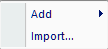
\includegraphics[keepaspectratio]{images/clipboard-478008996.png}}
    \texttt{Add} enables the user to manually draw either a point, line,
    or polygon ignition directly in \emph{Prometheus.}
    \texttt{Import...} allows the user to add an ignition file directly
    to the project that has been obtained / created elsewhere.
  \item
    If \texttt{Add} is used, select your desired ignition type:

    \begin{enumerate}
    \def\labelenumiii{\alph{enumiii}.}
    \tightlist
    \item
      \texttt{Point} ignition will start your fire growth from a
      specific point (or points) on the landscape.

      \begin{enumerate}
      \def\labelenumiv{\arabic{enumiv}.}
      \tightlist
      \item
        To add the \texttt{Point} left-click on a location in the map
        window and a red dot will appear.
      \item
        You can add as many or as few points as desired throughout the
        grid.
      \item
        Double left-click to finalize the points. A dialogue box will
        open.
      \item
        Name the ignition and set a start-time. Be specific with the
        start-time as this is a necessary component in conjunction with
        your weather stream.
      \end{enumerate}
    \item
      \texttt{Line} ignition will start your fire growth along the drawn
      line(s).

      \begin{enumerate}
      \def\labelenumiv{\arabic{enumiv}.}
      \tightlist
      \item
        To add the \texttt{Line} ignition, left-click on an area of the
        map and then move your cursor to where you want the line segment
        to end. Either double left-click to finalize this line ignition
        or single left-click to start a new segment line.
      \item
        A dialogue box will open. Name the ignition and mind the
        start-time.
      \end{enumerate}
    \item
      \texttt{Polygon} ignition will start your fire growth along the
      \emph{exterior} of the drawn polygon.

      \begin{enumerate}
      \def\labelenumiv{\arabic{enumiv}.}
      \tightlist
      \item
        Similar to the \texttt{Line} ignition above but you will need to
        finalize the connection of your last segment to the starting
        segment to create the polygon.
      \item
        Name the ignition and mind the start-time.
      \end{enumerate}
    \end{enumerate}
  \end{enumerate}
\item
  Save your project.
\end{enumerate}

\section{Scenario Set-up}\label{scenario-set-up}

This section covers setting up a \texttt{Scenario} from which to produce
a fire growth model output.

\begin{enumerate}
\def\labelenumi{\arabic{enumi}.}
\tightlist
\item
  Under the \texttt{Components} menu, select the \texttt{Scenarios}
  folder. An initial scenario will already exist in most cases. Either
  edit this or create a new scenario.
\item
  A \texttt{Scenario} dialogue box will open with multiple tabs and
  windows within it.

  \begin{enumerate}
  \def\labelenumii{\roman{enumii}.}
  \tightlist
  \item
    \texttt{Scenario\ Inputs} is the main tab.

    \begin{enumerate}
    \def\labelenumiii{\alph{enumiii}.}
    \tightlist
    \item
      Set the \texttt{Start\ Time:} and \texttt{End\ Time:} for your
      scenario. These should reflect the correct dates and times you
      wish to simulate, i.e.~\texttt{June\ 1,\ 2020\ 11:00} to
      \texttt{June\ 6,\ 2020\ 22:00}
    \item
      In the \texttt{Ignitions} window, use the check box to select the
      ignitions you wish to model. You can add more than one.
    \item
      If you have added \texttt{Fuel\ Breaks} you can activate those
      here.
    \item
      If you have added \texttt{Grid\ and\ Patches} you can activate
      those here at your discretion.
    \item
      Select your \texttt{Weather\ Stream}. We will return to this.
    \end{enumerate}
  \item
    \texttt{Burning\ Conditions} tab offers the user the ability to set
    under what conditions a fire can grow in the model.

    \begin{enumerate}
    \def\labelenumiii{\alph{enumiii}.}
    \tightlist
    \item
      The amount of rows will correspond to the total number of days you
      added in the above \texttt{Start\ Time:} and \texttt{End\ Time:}
      options (in our example, there would be six rows)
    \item
      \texttt{Start\ Time} under the \texttt{Burning\ Conditions} tab
      refers to the time at which a fire is enabled to spread on a given
      day.
    \item
      \texttt{End\ Time} under the \texttt{Burning\ Conditions} tab
      refers to the latest time at which a fire is enabled to spread on
      a given day.
    \item
      \texttt{HISI\ \textgreater{}} allows a user to define a threshold
      for \texttt{Initial\ Spread\ Index} at which a fire will begin
      spreading.

      \begin{enumerate}
      \def\labelenumiv{\alph{enumiv}.}
      \tightlist
      \item
        For example, \texttt{HISI\ \textgreater{}} set to a value of 5
        means that a fire will \emph{not} grow under any circumstances
        where the Hourly Initial Spread Index (\texttt{HISI}) is below
        5.
      \end{enumerate}
    \item
      \texttt{HFWI\ \textgreater{}} allows a user to define a threshold
      for \texttt{Fire\ Weather\ Index} at which a fire will begin
      spreading.

      \begin{enumerate}
      \def\labelenumiv{\alph{enumiv}.}
      \tightlist
      \item
        For example, \texttt{HFWI\ \textgreater{}} set to a value of 15
        means that a fire will \emph{not} grow under any circumstances
        where the Hourly Initial Spread Index (\texttt{HFWI}) is below
        15.
      \end{enumerate}
    \item
      \texttt{WS\ \textgreater{}} allows a user to define a threshold
      for \texttt{Wind\ Speed} at which a fire will begin spreading.

      \begin{enumerate}
      \def\labelenumiv{\alph{enumiv}.}
      \tightlist
      \item
        For example, \texttt{WS\ \textgreater{}} set to a value of 10
        means that a fire will \emph{not} grow under any circumstance
        when the \texttt{Wind\ Speed} is less than 10km/hr.
      \end{enumerate}
    \item
      \texttt{RH\ \textless{}} allows a user to define a threshold for
      \texttt{Relative\ Humidity}, at which a fire will begin spreading.

      \begin{enumerate}
      \def\labelenumiv{\alph{enumiv}.}
      \tightlist
      \item
        For example, \texttt{RH\ \textless{}} set to a value of 60 means
        that a fire will \emph{not} grow unless the
        \texttt{Relative\ Humidity} is lower than 60.
      \end{enumerate}
    \end{enumerate}
  \item
    \texttt{Fire\ Weather} tab offers the user the option to interpolate
    \texttt{Fire\ Weather} spatially. Three options exist. If you enable
    \texttt{Fire\ Weather\ Interpolation} you will need to return to
    \texttt{Scenario\ Inputs} tab and identify a primary weather stream.
  \item
    \texttt{Fire\ Behaviour} tab provides several options to refine
    various fire behaviour aspects.

    \begin{enumerate}
    \def\labelenumiii{\roman{enumiii}.}
    \tightlist
    \item
      \texttt{FMC\ (\%)\ override:} this adjusts the Foliar Moisture
      Content threshold.
    \item
      \texttt{Terrain\ effect} tells \emph{Prometheus} to consider
      topography provided for wind.
    \item
      \texttt{Breaching} enables fire to breach \texttt{Fuel\ Breaks} if
      enabled and a fuel break is provided.
    \item
      \texttt{Spotting} does nothing and should not be available to
      enable/disable.
    \item
      \texttt{Percentile\ rate\ of\ spread:} ???
    \item
      \texttt{Green-up} allows the user to set the \texttt{Start\ Date:}
      and \texttt{End\ Date} periods for where the model should use the
      \texttt{Green} fuel type models.
    \item
      \texttt{Standing\ Grass} allows the user to set the
      \texttt{Start\ Date} and \texttt{End\ Date} for where the model
      should use \texttt{Standing} versus \texttt{Matted} grass models.
    \item
      \texttt{Grass\ Curing} section allows a user to set the
      \texttt{Degree\ of\ Curing\ (\%)} across the grid. It further
      enables the user to dynamically set dates for curing over time.
    \end{enumerate}
  \item
    \texttt{Propagation} tab provides several additional options that
    affect model performance and outputs.

    \begin{enumerate}
    \def\labelenumiii{\roman{enumiii}.}
    \tightlist
    \item
      \texttt{Display\ interval} will default to \texttt{01:00:00} but
      this can be adjusted at the user discretion. an interval of
      \texttt{01:00:00} will display fire growth every hour. Can be
      lowered or increased depending on desire.
    \item
      \texttt{Maximum\ time\ step\ during\ acceleration:} defaults to
      \texttt{00:02:00} which is a two-minute interval time step. This
      is rarely needed to be adjusted.
    \item
      \texttt{Stop\ fire\ spread\ at\ data\ boundary} will stop your
      fire from ``spreading'' beyond the extent of the fuel data.
    \item
      \texttt{Purge\ non-displayable\ time\ steps} ???
    \item
      \texttt{Fire\ may\ grow\ with\ independent\ time\ steps} useful
      for when you have multiple ignitions in one scenario.
    \end{enumerate}
  \item
    Once all settings are set and verified, click \texttt{OK}.
  \item
    Save your project.
  \item
    You are now ready to \texttt{Run} the model!
  \end{enumerate}
\end{enumerate}

\bookmarksetup{startatroot}

\chapter{Introduction}\label{introduction}

This book is intended as an unofficial user-guide for the
\emph{Prometheus} fire growth modelling software, specific to version
2023.06.01, as of June 1st, 2023. This is the End of Life (EOL) version
and final officially released version of the software. In this book, we
will cover breadth of topics related to \emph{Prometheus}, with the goal
of enabling broader usage of this tool and to catalogue the known but
unwritten issues, bugs, errors, and outright confusing aspects of the
software. \emph{Prometheus} is and has been a valuable tool for Canadian
wildland fire\footnote{While many terms, I choose to use wildland fire.
  Forest fire, brush fire, bush fire, wildfire, grass fire, whatever
  term you prefer, I am generally referring to that.} managers since its
initial release, and we expect that it will continue to be used many
years into the future, despite newer and more impactful software being
developed. However, it is also possible that \emph{Prometheus} usage
will entirely disappear in an operational and research context in the
near future. In either case, it will be important to document and
describe how this software functioned, how to use it, and most
critically, how to resolve the myriad issues inherent to
\emph{Prometheus}.

\emph{Prometheus} is a deterministic wildland fire growth modelling
software that is based around the \emph{Canadian Forest Fire Danger
Rating System (CFFDRS),} utilizing the \emph{Fire Weather Index (FWI)}
and the \emph{Fire Behaviour Prediction (FBP)} systems to predict
potential fire growth. This text will assume the reader is well-versed
in the FWI and FBP systems with a broad understanding of both the
limitations and inherent assumptions of the CFFDRS\footnote{If you are
  unfamiliar with the CFFDRS and it's sub-systems FWI and FBP, we
  strongly suggest reading the background literature before proceeding
  with \emph{Prometheus} usage. A thorough understanding will improve
  both results and your eventual work in fire growth modelling.}. Some
aspects of interpretation of \emph{Prometheus}, weather, fire weather,
and other related aspects will be present in this text, however we
expect that all readers will have some baseline knowledge.

Specialized training in fire behaviour is \textbf{not} a requirement for
using \emph{Prometheus.} We encourage anyone with an interest in
wildland fire to use and work with fire growth modelling software. While
many aspects of \emph{Prometheus} will feel more intuitive to those with
prior training and experience in wildland fire, the basic concepts can
be learned through a variety of resources, including \emph{Prometheus}
itself as a tool for learning about the CFFDRS.

\emph{Prometheus} doesn't strictly require any coding or geospatial
training or knowledge, but it is a definite benefit. Throughout this
text, we will include code snippets and instructions that may rely on
additional software and tools. These are \emph{not} required, but
greatly streamline the \emph{Prometheus} workflow and better enable
effective manipulation of the software itself.

We strongly suggest readers install and familiarize themselves with
\emph{R} and \emph{QGIS}. Both are open-source and very powerful tools.
We also recommend the use of \emph{RStudio,} especially for individuals
who are newer to programming in general. While we also recommend
additional learning for both \emph{R} and \emph{QGIS}, we will provide
code with instructions that the majority of readers will be able to use
without prior knowledge.

\emph{Prometheus} requires a variety of datasets to operate, with
further additional data inputs that can improve and refine a model, but
aren't strictly required. We will provide options for obtaining and/or
creating necessary input data from open-access sources. Most of these
sources will rely on national datasets from the Canadian Forest Service
(CFS).

Lastly, while we call this a \emph{user-guide} we also wish to emphasize
that this guide is not intended to cover every single aspect, nor should
one expect it to cover specific aspects of older file types. We will
refer to the most common usage of files and file types in current use.
For example, fuel type layers will be discussed in the \textbf{GeoTiff}
format primarily.

\bookmarksetup{startatroot}

\chapter{Installation \& Set-up}\label{installation-set-up}

\emph{Prometheus} is free software that anyone can install with the
correct computer. Obtain the necessary files here:
\url{https://firegrowthmodel.ca/\#/prometheus_software}.
\emph{Prometheus} can operate on most Windows based computers, with
verified functionality on Windows Vista - Windows 11.

Please take some time to read this website, specifically the
\emph{Prometheus} software sections. Some useful documentation can be
found under the Documentation page.

\emph{Prometheus} can be run on the vast majority of personal computers
and does not require a powerful workstation to function. Depending on
what you aim to use the software for, the software may become less
performant. Very complex fire simulations with heavy data will reduce
software performance and can greatly overtax your computer. Be mindful
of what you do; the software will run what you ask of it.

A few additional installations are required in advance of
\emph{Prometheus} set-up. A specific Intel Redist (which is a set of
runtime library files) is required for \emph{Prometheus} to
function\footnote{Intel hardware is \textbf{not} required for
  \emph{Prometheus}, the Intel Redist is not hardware locked.}. In
addition, a Java Runtime is required (v1.8.0) and can be obtained here:
\url{https://www.java.com/en/download/manual.jsp}

\emph{Prometheus} requires a specific \textbf{Intel Redist
version\emph{.}} The software will not be installed without this and the
user is required to ensure this is present on their machine. The correct
version can be found on the firegrowthmodel.ca website currently. The
required file is \textbf{Intel C++ runtime 2021.3.0.3372.}

This is a hard requirement. You cannot bypass this requirement and run
\emph{Prometheus}.

During installation of \emph{Prometheus,} if either requirement is not
found, the installation will not continue. It is also suggested that the
user reboot their computer \emph{after} installation of both the Java
and Intel components and prior to completing \emph{Prometheus}
installation.

\section{Verify Path Settings}\label{verify-path-settings}

Post-installation, check and verify what path has been set for the
\emph{Prometheus} software. \emph{Prometheus} has known conflicts,
notably with other installations of GDAL, which can lead to frustrating
and unclear issues. On a Windows machine, press the Windows key or the
Windows icon to open the search bar. Type,\\
``Environment'' and two options should populate, ``\emph{Edit the system
environment variables.''} or \emph{``Edit environment variables for your
account.''}

Administrative privileges may be required depending on your
user/corporate settings to view and edit environment variables. You
should see a window similar to this,

\pandocbounded{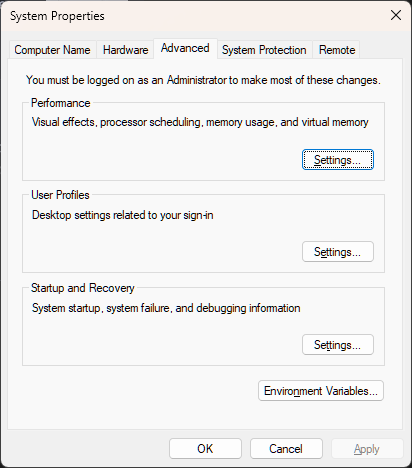
\includegraphics[keepaspectratio]{images/clipboard-590267188.png}}

Select the \textbf{Environment Variables} option near the bottom right.
A window similar to this should open,

\pandocbounded{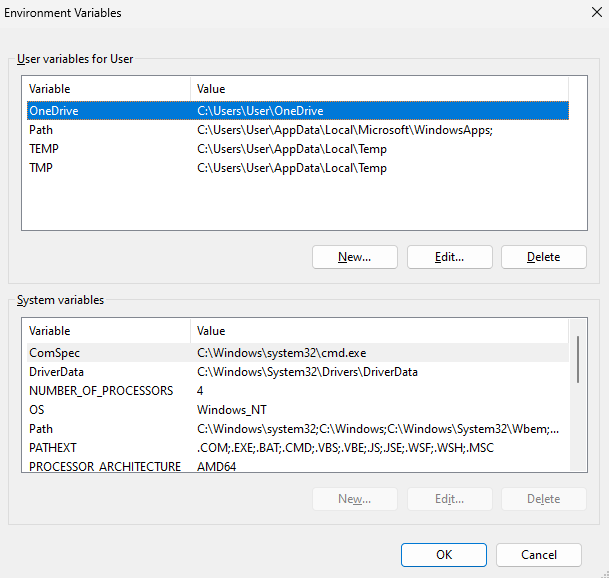
\includegraphics[keepaspectratio]{images/clipboard-666687807.png}}

In the \textbf{System Variables} section, look for the \emph{Variable}
\texttt{GDAL\_DATA} first. The \emph{Value} should be similar to,\\
\texttt{C:\textbackslash{}Program\ Files\textbackslash{}Prometheus\textbackslash{}gdal-data\textbackslash{}}

Verify that this is correctly set. Next, search in the same list for the
\emph{Variable} \texttt{PROJ\_LIB}. The \emph{Value} should be similar
to,

\texttt{C:\textbackslash{}Program\ Files\textbackslash{}Prometheus\textbackslash{}proj\_nad\textbackslash{}}

Verify that this is correctly set. If so, \emph{Prometheus} should be
ready for usage.

\subsection{Troubleshooting Paths}\label{troubleshooting-paths}

In some cases, both \texttt{GDAL\_DATA} and \texttt{PROJ\_LIB} may point
to other paths, such as an \texttt{OSGEO} installation as a part of
QGIS. In order to properly utilize both \emph{Prometheus} and other
spatial software, the user may occasionally be required to re-direct the
path destination directly. If either \texttt{GDAL\_DATA} or
\texttt{PROJ\_LIB} are elsewhere, we recommend you copy those locations
to a separate text file for future use and update them to be the
required \emph{Prometheus} paths noted above (ensure your directories
are aligned).

\bookmarksetup{startatroot}

\chapter{Input Data: Gathering and
Formatting}\label{input-data-gathering-and-formatting}

Generally, a successful fire growth model will require several inputs to
properly operate. The common inputs are: fuel data, weather data, and
topography data. In \emph{Prometheus}, these are represented as either
raster or vector based data. A variety of possible inputs and file
formats exist for \emph{Prometheus:}

\begin{enumerate}
\def\labelenumi{\arabic{enumi}.}
\tightlist
\item
  Landscape / Topographic

  \begin{enumerate}
  \def\labelenumii{\roman{enumii}.}
  \tightlist
  \item
    Fuel Data

    \begin{enumerate}
    \def\labelenumiii{\alph{enumiii}.}
    \tightlist
    \item
      Fuel data for \emph{Prometheus} must be in raster format and
      follow a specific fuel assignment as a default. The user can
      supply a Fuel Look-Up Table (LUT) if their raster data follows a
      different format.

      \begin{enumerate}
      \def\labelenumiv{\alph{enumiv}.}
      \setcounter{enumiv}{1}
      \tightlist
      \item
        \emph{Fuel Patches} are an optional input that will be covered
        in further detail below.
      \end{enumerate}
    \end{enumerate}
  \item
    Elevation Data

    \begin{enumerate}
    \def\labelenumiii{\alph{enumiii}.}
    \tightlist
    \item
      Elevation data for \emph{Prometheus} must be in raster format.
      Generally, a user will obtain a Digital Elevation Model (DEM) or
      similar product to represent the topography in their landscape.
    \end{enumerate}
  \item
    Slope \& Aspect Data

    \begin{enumerate}
    \def\labelenumiii{\roman{enumiii}.}
    \tightlist
    \item
      Slope and Aspect grids can both be provided if desired for usage
      in \emph{Prometheus.} They must match the same format and extent
      of the Fuel and Elevation data.
    \end{enumerate}
  \item
    Degree of Curing (\%)

    \begin{enumerate}
    \def\labelenumiii{\roman{enumiii}.}
    \tightlist
    \item
      A Grid containing percent curing values. This grid must be of the
      same extent and format as the Fuel layer. This is primarily used
      to influence Grass fire behaviour through curing estimates.
    \end{enumerate}
  \item
    Green-Up

    \begin{enumerate}
    \def\labelenumiii{\roman{enumiii}.}
    \tightlist
    \item
      A grid that denotes whether a given cell should be labeled
      ``Green''. This is generally applied for the D-1 Leafless Aspen,
      M-1 Mixedwood-Leafless, and M-3, Dead Balsam Fir
      Mixedwood--Leafless fuel types, indicating that they should
      instead utilize the D-2 Green Aspen, M-2 Mixedwood-Green, and the
      M-4 Dead Balsam Fir Mixedwood--Green fuel types, respectively.
    \end{enumerate}
  \item
    Percent Conifer

    \begin{enumerate}
    \def\labelenumiii{\roman{enumiii}.}
    \tightlist
    \item
      Optional input that can be used to refine the Mixedwood
      classification.
    \end{enumerate}
  \item
    Percent Dead Fir

    \begin{enumerate}
    \def\labelenumiii{\roman{enumiii}.}
    \tightlist
    \item
      Optional input that can be used to refine the Dead Balsam Fir
      Mixedwood fuel types.
    \end{enumerate}
  \item
    Crown Base Height

    \begin{enumerate}
    \def\labelenumiii{\roman{enumiii}.}
    \tightlist
    \item
      These data specifically operate for the C-6 Conifer Plantation
      fuel type and can be used to better adjust and refine fire
      behaviour in these fuels where data exists.
    \end{enumerate}
  \item
    Tree Height

    \begin{enumerate}
    \def\labelenumiii{\roman{enumiii}.}
    \tightlist
    \item
      ?
    \end{enumerate}
  \item
    Fuel Load

    \begin{enumerate}
    \def\labelenumiii{\roman{enumiii}.}
    \tightlist
    \item
      ?
    \end{enumerate}
  \end{enumerate}
\item
  Weather / Meteorological

  \begin{enumerate}
  \def\labelenumii{\roman{enumii}.}
  \tightlist
  \item
    Weather Station

    \begin{enumerate}
    \def\labelenumiii{\alph{enumiii}.}
    \tightlist
    \item
      Weather stations are manually added to the project in
      \emph{Prometheus}. By default, a new weather station will be
      placed at the center of your project data geographically, but can
      be altered through adjusting the coordinates. Weather stations can
      be added that do not fall within the extent of your project data.
    \item
      Weather stations are how the user inputs weather streams to
      provide weather inputs for use in the fire growth model.
    \item
      Weather streams will be covered in more depth in the
      \textbf{\emph{Weather Section}}.
    \end{enumerate}
  \item
    Weather Patches \& Weather Grids

    \begin{enumerate}
    \def\labelenumiii{\roman{enumiii}.}
    \tightlist
    \item
      Weather patches and grids are utilized to better model and reflect
      topographical influence on wind in \emph{Prometheus.} Patches
      represent smaller areas for better modelling while weather grids
      are built off of the elevation data and must match the input
      elevation layer extent. Weather grids can be created through the
      usage of the \emph{Wind Ninja} software, which will be covered in
      a later section for advanced usage.
    \end{enumerate}
  \end{enumerate}
\item
  Ignition Data

  \begin{enumerate}
  \def\labelenumii{\roman{enumii}.}
  \tightlist
  \item
    Several options exist to input ignitions in \emph{Prometheus.} The
    user can manually draw and add either point, line, or polygon
    ignitions natively within \emph{Prometheus} or they can upload data
    directly from other sources in point, line, or polygon format, but
    the data must be in a vector format.

    \begin{enumerate}
    \def\labelenumiii{\alph{enumiii}.}
    \tightlist
    \item
      \emph{Prometheus} accepts Shapefile (.shp) and Keyhole Markup
      Language / Keyhole Markup Zipped (.kml, .kmz) file types for
      ignition data.
    \end{enumerate}
  \end{enumerate}
\end{enumerate}

At an absolute minimum, \emph{Prometheus} requires a raster Fire
Behaviour Prediction (FBP) Fuel Type (FT) input layer (we will use the
term fuel layer from here out). Three file formats are accepted for
raster data in \emph{Prometheus:} GeoTIFF (.tif, .tiff), ASCII (.asc),
and text (.txt). The most common file type that users will encounter is
a standard GeoTIFF, which is the most common raster format in present
geospatial usage. There are several options to obtain or create a fuel
layer for usage in \emph{Prometheus.} Some specific requirements must be
met otherwise the layer will not be imported correctly.

Throughout the next sections, we will describe how to obtain and format
data for usage in \emph{Prometheus.}

\section{Fuel Data}\label{fuel-data}

Obtaining fuel data for \emph{Prometheus} is currently easier and more
accessible than ever, though this data is not always the best available
due to a variety of challenges and limitations. The Canadian Forest
Service (CFS) produces a national Fire Behaviour Prediction (FBP) Fuel
Type (FT) layer for all of Canada, which is what we will cover in this
section. This layer is based on remotely sensed data and is developed
through a rule-set application to attempt to best reflect expected fire
behaviour in Canada. Other fuel type datasets exist but are often not
easily accessible. The basic concepts covered in this section will apply
for the creation and usage of other fuel type data where a user may have
it available.

\subsection{Obtaining Fuel Data via R}\label{obtaining-fuel-data-via-r}

\bookmarksetup{startatroot}

\chapter*{References}\label{references}
\addcontentsline{toc}{chapter}{References}

\markboth{References}{References}

\protect\phantomsection\label{refs}




\end{document}
